\subsection{Computing Exact Trigonometric Ratios}
The \dfont{unit circle} is often used to determine the \ifont{exact} value of a particular trigonometric function.

$$
\includegraphics[width=5in]{images/unit-circle}$$

Reading from the unit circle one can see that $\cos 5\pi/6=-\sqrt 3/2$ and $\sin 5\pi/6=1/2$ (remember the that the $x$-coordinate is $\cos\theta$ and the $y$-coordinate is $\sin\theta$).
However, we don't always have access to the unit circle.
In this case, we can compute the exact trigonometric ratios for $\theta=5\pi/6$ by using \dfont{special triangles} and the \dfont{CAST rule} described below.

The first special triangle has angles of $45^\circ,45^\circ,90^\circ$ (i.e., $\pi/4,\pi/4,\pi/2$) with side lengths $1,1,\sqrt 2$, while the second special triangle has angles of $30^\circ,60^\circ,90^\circ$ (i.e., $\pi/6,\pi/3,\pi/2$) with side lengths $1,2,\sqrt 3$. They are classically referred to as the $1-1-\sqrt{2}$ triangle, and the $1-2-\sqrt{3}$ triangle, respectively, shown below.
$$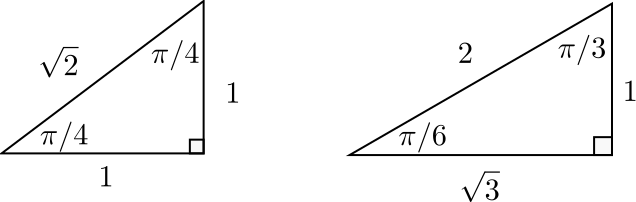
\includegraphics[width=4.0in]{images/trig4}$$

\begin{formulabox}[Mnemonic]
The first triangle should be easy to remember. 
To remember the second triangle, place the largest number ($2$) across from the largest angle ($90^\circ=\pi/2$).
Place the smallest number ($1$) across from the smallest angle ($30^\circ=\pi/6$).
Place the middle number ($\sqrt 3\approx 1.73$) across from the middle angle ($60^\circ=\pi/3$).
Double check using the Pythagorean Theorem that the sides satisfy $a^2+b^2=c^2$.
\end{formulabox}

The special triangles allow us to compute the exact value (excluding the sign) of trigonometric ratios, but to determine the sign, we can use the \ifont{CAST rule}.

\begin{formulabox}[The CAST Rule]
The CAST rule says that in quadrant I all three of $\sin\theta$, $\cos\theta$, $\tan\theta$ are positive.
In quadrant II, only $\sin\theta$ is positive, while $\cos\theta$, $\tan\theta$ are negative.
In quadrant III, only $\tan\theta$ is positive, while $\sin\theta$, $\cos\theta$ are negative.
In quadrant IV, only $\cos\theta$ is positive, while $\sin\theta$, $\tan\theta$ are negative. 
To remember this, simply label the quadrants by the letters C-A-S-T starting in the bottom right and labelling counter-clockwise.
\end{formulabox} 

$$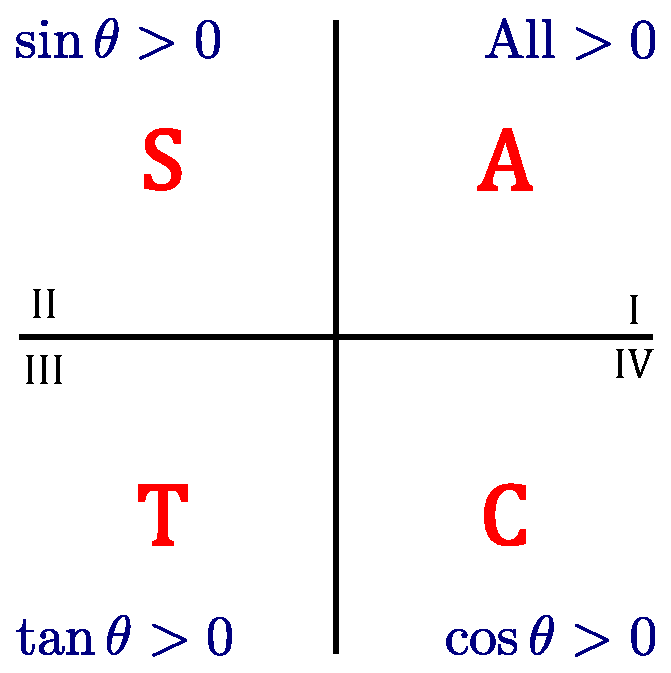
\includegraphics[width=2.5in]{images/trig5}$$

\begin{example}{Determining Trigonometric Ratios Without Unit Circle}{CASTRule}
Determine $\sin 5\pi/6$, $\cos 5\pi/6$, $\tan 5\pi/6$, $\sec 5\pi/6$, $\csc 5\pi/6$ and $\cot 5\pi/6$ exactly by using the special triangles and CAST rule.
\end{example}

\begin{solution} 
We start by drawing the $xy$-plane and indicating our angle of $5\pi/6$ in standard position (positive angles rotate \ifont{counterclockwise} while negative angles rotate \ifont{clockwise}).
Next, we drop a perpendicular to the $x$-axis (never drop it to the $y$-axis!).
$$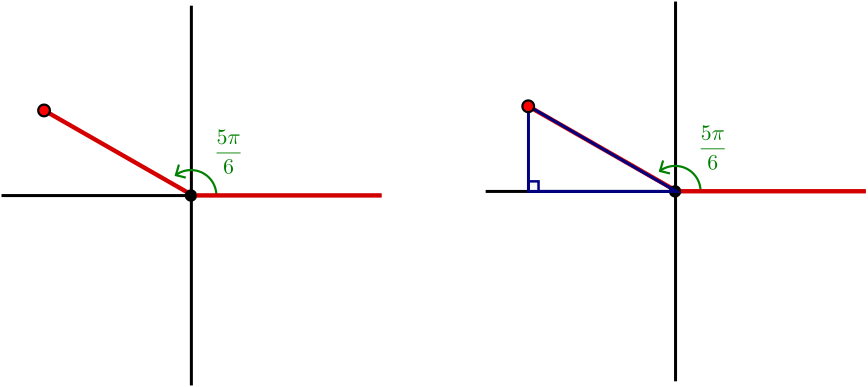
\includegraphics[width=4in]{images/trig6}$$
Notice that we can now figure out the angles in the triangle.
Since $180^\circ=\pi$, we have an interior angle of $\pi-5\pi/6=\pi/6$ inside the triangle. 
As the \ifont{angles of a triangle add up to $180^\circ=\pi$}, the other angle must be $\pi/3$. 
This gives one of our special triangles.
We label it accordingly and add the CAST rule to our diagram.
$$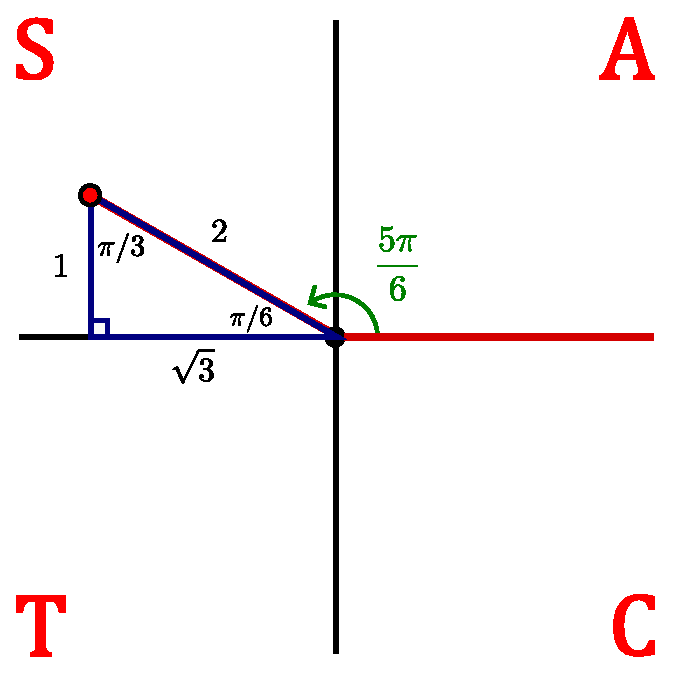
\includegraphics[width=3in]{images/trig7}$$
From the above figure we see that $5\pi/6$ lies in quadrant II where $\sin\theta$ is positive and $\cos\theta$ and $\tan\theta$ are negative.
This gives us the \ifont{sign} of $\sin\theta$, $\cos\theta$ and $\tan\theta$.
To determine the \ifont{value} we use the special triangle and SOH CAH TOA.

Using $\sin\theta=opp/hyp$ we find a value of $1/2$.
But $\sin\theta$ is positive in quadrant II, therefore, 
$$\sin \frac{5\pi}{6}=+\frac{1}{2}.$$

Using $\cos\theta=adj/hyp$ we find a value of $\sqrt 3/2$.
But $\cos\theta$ is negative in quadrant II, therefore, 
$$\cos \frac{5\pi}{6}=-\frac{\sqrt 3}{2}.$$

Using $\tan\theta=opp/adj$ we find a value of $1/\sqrt 3$.
But $\tan\theta$ is negative in quadrant II, therefore, 
$$\tan \frac{5\pi}{6}=-\frac{1}{\sqrt 3}.$$

To determine $\sec\theta$, $\csc\theta$ and $\cot\theta$ we use the definitions:
$$\csc \frac{5\pi}{6} = \ds\frac{1}{\sin \frac{5\pi}{6}} = +2,
\qquad \sec \frac{5\pi}{6} = \ds\frac{1}{\cos \frac{5\pi}{6}} = -\frac{2}{\sqrt 3},
\qquad\cot \frac{5\pi}{6} = \ds\frac{1}{\tan \frac{5\pi}{6}} = -\sqrt 3.$$
\end{solution}

\begin{example}{CAST Rule}{CASTRule2}
If $\cos\theta=3/7$ and $3\pi/2<\theta< 2\pi$, then find $\cot\theta$.
\end{example}

\begin{solution} 
We first draw a right angle triangle.
Since $\cos\theta=adj/hyp=3/7$, we let the adjacent side have length $3$ and the hypotenuse have length $7$.
$$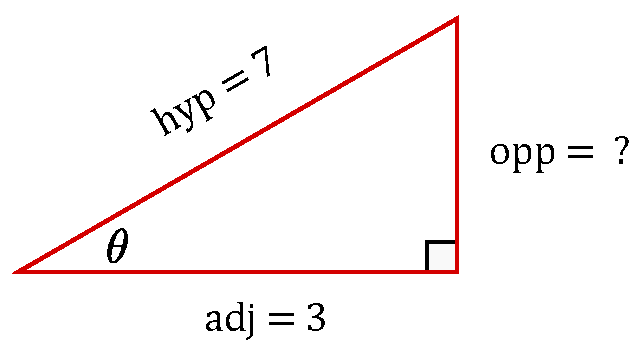
\includegraphics[height=1.1in]{images/trig8}$$
Using the Pythagorean Theorem, we have $3^2+(\mbox{opp})^2=7^2$.
Thus, the opposite side has length $\sqrt{40}$.
$$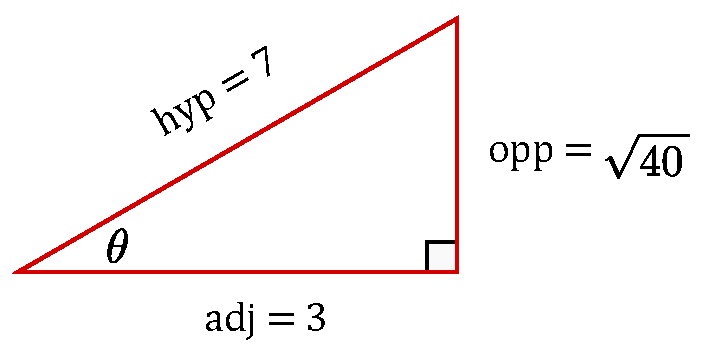
\includegraphics[height=1.1in]{images/trig9}$$
%Recall that \green{right angle triangles} can give us the \red{value} of trigonometric ratios while the \green{CAST rule} gives us the \red{sign}.**
To find $\cot\theta$ we use the definition:
$$\cot\theta=\frac{1}{\tan\theta}.$$
Since we are given $3\pi/2<\theta< 2\pi$, we are in the fourth quadrant. By the CAST rule, $\tan\theta$ is negative in this quadrant.
As $\tan\theta=opp/adj$, it has a value of $\sqrt{40}/3$, but by the CAST rule it is negative, that is,
$$\tan\theta=-\frac{\sqrt{40}}{3}.$$
Therefore,
$$\cot\theta=-\frac{3}{\sqrt{40}}.$$
\end{solution}